\documentclass{article}
\usepackage{graphicx}
\usepackage{amsmath}
\usepackage{xspace}
\usepackage{hyperref}

% System name: use \sys everywhere in the body for a consistent small-caps mark.
\newcommand{\sys}{\textsc{ScanStudio}\xspace}

\title{ScanStudio: Video to PDF for Document Intelligence}

\author{Erick Duarte, Akshit Jain, Rohan Boddu,\\Rolando Garcia, Tyson Winarski, Ross Maciejewski}

\begin{document}

\maketitle

% NOTE: In the full paper this is Section 3, following the Introduction,
% Background, and Related Work. The counter is bumped so the standalone
% preview also numbers it 3; remove this line when merging.
\setcounter{section}{2}

\section{ScanStudio}
\label{sec:scanstudio}

\sys turns physical documents---whether bound books or stacks of loose
paperwork such as intake forms or receipts---into clean, page-separated PDFs as
the operator simply flips through them. The operator points a consumer webcam at
a document like a scanning head (Figure~\ref{fig:rig}); \sys records the session
and, in real time, captures one sharp image of each spread the moment the pages
settle after a turn. Each capture is confirmed on-the-fly: a chime and a green
\texttt{CAPTURED} badge flash the instant a frame is committed, so the operator
always knows, spread by spread, what the system has captured (and what it has not).
Because capture and frame selection happen in a single pass, with no separate
offline stage to launch and wait on, the page images are ready the moment the
operator sets the book down. 
The capture hardware is deliberately minimal, a webcam clamped to a well-lit desk, 
and a single command carries the result through to a finished document.

This live path is \sys's primary capture mode, and it keeps the operator in a
tight control loop: real-time feedback lets them adjust their pace 
and fix mistakes as they go (Section~\ref{sec:live}). For footage shot away from a
workstation, \sys also accepts a pre-recorded video and recovers the same
per-spread keyframes in a batch pass (Section~\ref{sec:offline}). Both paths emit
identical artifacts: one full-resolution keyframe per spread plus its
metadata, so the shared back end reviews, crops, splits, and assembles the final
PDF the same way, regardless of how the keyframes were captured.
Figure~\ref{fig:pipeline} shows the full pipeline: the orange stages are the front
end (run live during capture), the green stages the corresponding back half.

\begin{figure}[t!]
    \centering
    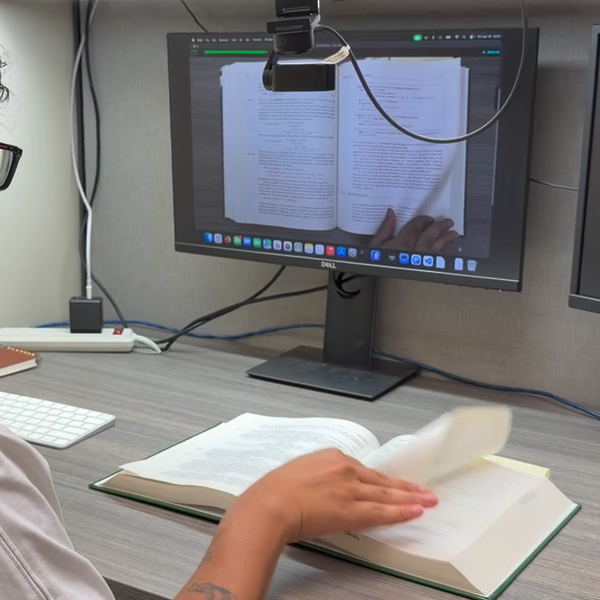
\includegraphics[width=0.97\columnwidth]{images/OverheadRig.png}
    \caption{The overhead digitization rig. A 4K webcam is mounted above a
    well-illuminated workspace; real-time alignment and quality control are
    monitored on screen as the operator turns pages.}
    \label{fig:rig}
\end{figure}

\begin{figure*}[t!]
    \centering
    \includegraphics[width=0.95\linewidth]{images/video2pdf.png}
    \caption{The \sys pipeline. In live capture (\texttt{make live}), a fixed
    overhead camera films an operator turning pages while an online state machine
    tracks inter-frame motion and auto-captures the sharpest frame each time the
    book settles after a turn---the orange front-end stages, all running in real
    time. The same per-spread keyframes can instead be recovered offline (P1--P3)
    from a pre-recorded video. Either way, the green back half
    (\texttt{make finish}) is shared: an interactive review stage where the
    operator corrects the keyframe set and per-spread split geometry, followed by
    automated crop, split, and PDF assembly.}
    \label{fig:pipeline}
\end{figure*}

\subsection{The Overhead Rig}
\label{sec:capture}

We capture overhead video of a person flipping through pages with a 4K
Insta360 Link~2 webcam clamped to a standard reading light
(Figure~\ref{fig:rig}). Video is recorded at 24 frames per second with
autofocus enabled, which keeps individual frames sharp as the page settles. The
guiding principle is replicability: nothing about the hardware or lighting
should require specialized equipment. Accordingly, the rig also accommodates
all-in-one action cameras such as GoPros, smartphones on a stand, and other
high-resolution handheld devices.

Three conditions are critical for consistent capture:
\begin{itemize}
    \item \textbf{Lighting:} clear, even illumination from a desk lamp or
    overhead light, avoiding glare and hard shadows.
    \item \textbf{Frame quality:} at least 4K resolution, so that small
    characters remain legible after cropping.
    \item \textbf{Hands-free operation:} a steady mount or clamp, so the
    operator can turn pages naturally without holding or operating anything
    else.
\end{itemize}

Each requirement can be relaxed at the cost of additional technical machinery.
Less controlled lighting could be handled with adaptive histogram
equalization~\cite{pizer1987adaptive} or low-light denoising
models~\cite{li2015low}; camera movement could be tolerated with real-time
stabilization~\cite{castillo2004real} or motion-compensated frame
selection~\cite{huang2009correlation}; and hands-free operation could be
extended to wearables and AR headsets~\cite{mann1997wearable,
Meta2023RayBanMeta}. These are promising directions for future work.

\subsection{Live Keyframe Selection}
\label{sec:live}

In its primary mode, \sys selects keyframes \emph{live}, as the operator turns
pages. The webcam feed is recorded and analyzed at the same time: the system
tracks the page-turn rhythm and auto-captures one sharp frame per spread the
instant the book settles after a turn. Selection happens during the flip-through
itself, not in a later pass over the recording, so the page images are complete the
moment the operator closes the book. Throughout, the operator stays inside 
a tight feedback loop: a live motion bar and a capture chime
report what the system is doing, so its pace can be adjusted and a bad capture
corrected without having to exit the live view.

\noindent\textbf{Motion as a page-turn signal.}
\sys keys on the fact that page turns leave a distinctive signature in the video.
When a hand enters the frame and lifts a page, pixels change sharply from one
frame to the next: the page and hand move toward the camera (briefly defocusing),
and their shadows darken the book and table. When the page lies flat again,
successive frames are nearly identical. The feed therefore alternates between
bursts of high inter-frame motion (page turns) and quiet intervals (settled
spreads), and the quiet intervals are exactly where a clean, in-focus image of
each spread can be found. Concretely, let $I_t$ be frame $t$ downsampled to
360-pixel height and converted to grayscale; \sys computes the mean absolute
inter-frame difference
\begin{equation}
    m_t = \frac{1}{|\Omega|} \sum_{x \in \Omega} \bigl| I_t(x) - I_{t-1}(x) \bigr|,
    \label{eq:motion}
\end{equation}
over the pixel grid $\Omega$ on every incoming frame, smoothed online by a
trailing mean over the last $15$ frames so that thresholding is stable without
look-ahead. Computing it at reduced resolution keeps the analysis comfortably
within the per-frame budget.

\noindent\textbf{Online state machine.}
A three-state machine turns this signal into capture decisions in real time. From
\textsc{waiting}, a sustained drop below the settle threshold (a short run of
consecutive still frames) fires the first capture and moves to \textsc{settled}.
From \textsc{settled}, motion rising above the turn threshold signals a page turn
in progress and moves to \textsc{turning}. From \textsc{turning}, the next
sustained settle fires a capture and returns to \textsc{settled}. The settle and
turn thresholds straddle the quiet-interval and page-turn motion regimes
(Figure~\ref{fig:peaks}), and requiring the stillness to persist for a short dwell
time before capturing prevents a momentary pause mid-turn from triggering a
premature frame. The machine is causal---it decides from past frames alone and
cannot revise a capture after the fact---which is exactly what makes the operator
feedback loop below worth closing.

\noindent\textbf{Sharpest-of-window capture.}
Rather than grabbing the single frame at which the settle condition is met, \sys
keeps a short rolling buffer of recent frames and, on a capture event, commits the
\emph{sharpest} frame in the buffer (by variance of the Laplacian over its central
crop). The captured image is therefore the crispest instant of the settle, not
merely its leading edge.

\noindent\textbf{Keeping the capture loop real-time.}
Encoding 4K video in software is expensive enough to stall a naive
capture-and-display loop, so \sys offloads encoding to a background thread fed
through a bounded queue. The capture loop hands off each frame and returns
immediately to preview and analysis, while the encoder drains the queue at its
own pace. Because the queue is fixed in size, an encoder that falls behind
throttles capture---a brief, bounded stall---rather than piling up un-encoded
frames in unbounded memory; under load, frames are delayed, never dropped. A single downscale of each
4K frame feeds both the on-screen preview and the 360-pixel analysis frame,
avoiding a second pass over the full-resolution array. The heads-up display---a live motion bar with the settle and turn thresholds
marked, the current state, a running capture count, and a green
\texttt{CAPTURED} badge that flashes on each commit---occupies a band
\emph{above} the frame, so it never occludes the page (the orange pane in
Figure~\ref{fig:pipeline}). It is shown only on the operator's screen and is
never written to the recording, which stores only raw frames.

\noindent\textbf{A human in the control loop.}
The on-screen feedback and the per-capture chime close the loop around the operator
as much as around the software. At the immediate level, the operator can
force-capture the current frame, undo the last capture, and pause or resume
auto-capture without looking away from the book. More interestingly, the feedback
reshapes behavior on its own: operators quickly learn to pause briefly after each
turn and to flip more deliberately, and when an expected chime fails to sound---a
spread the detector missed---they will wave a hand over the page to mimic a turn and
coax out the capture, bending their own motions to fit the interface. This raises
both the page-flip rate and frame crispness with no change to the system
itself---the capture process effectively trains its own operator. Whether this self-serialization can be deliberately
cultivated, closing the gap with richer feedback rather than a better algorithm,
is an intriguing direction for future study. On exit, \sys writes the recording
alongside the keyframe images and their metadata, the same artifacts the offline
path produces, so the shared back half (Section~\ref{sec:backhalf}) proceeds
identically.

% \begin{figure*}[t!]
%     \centering
%     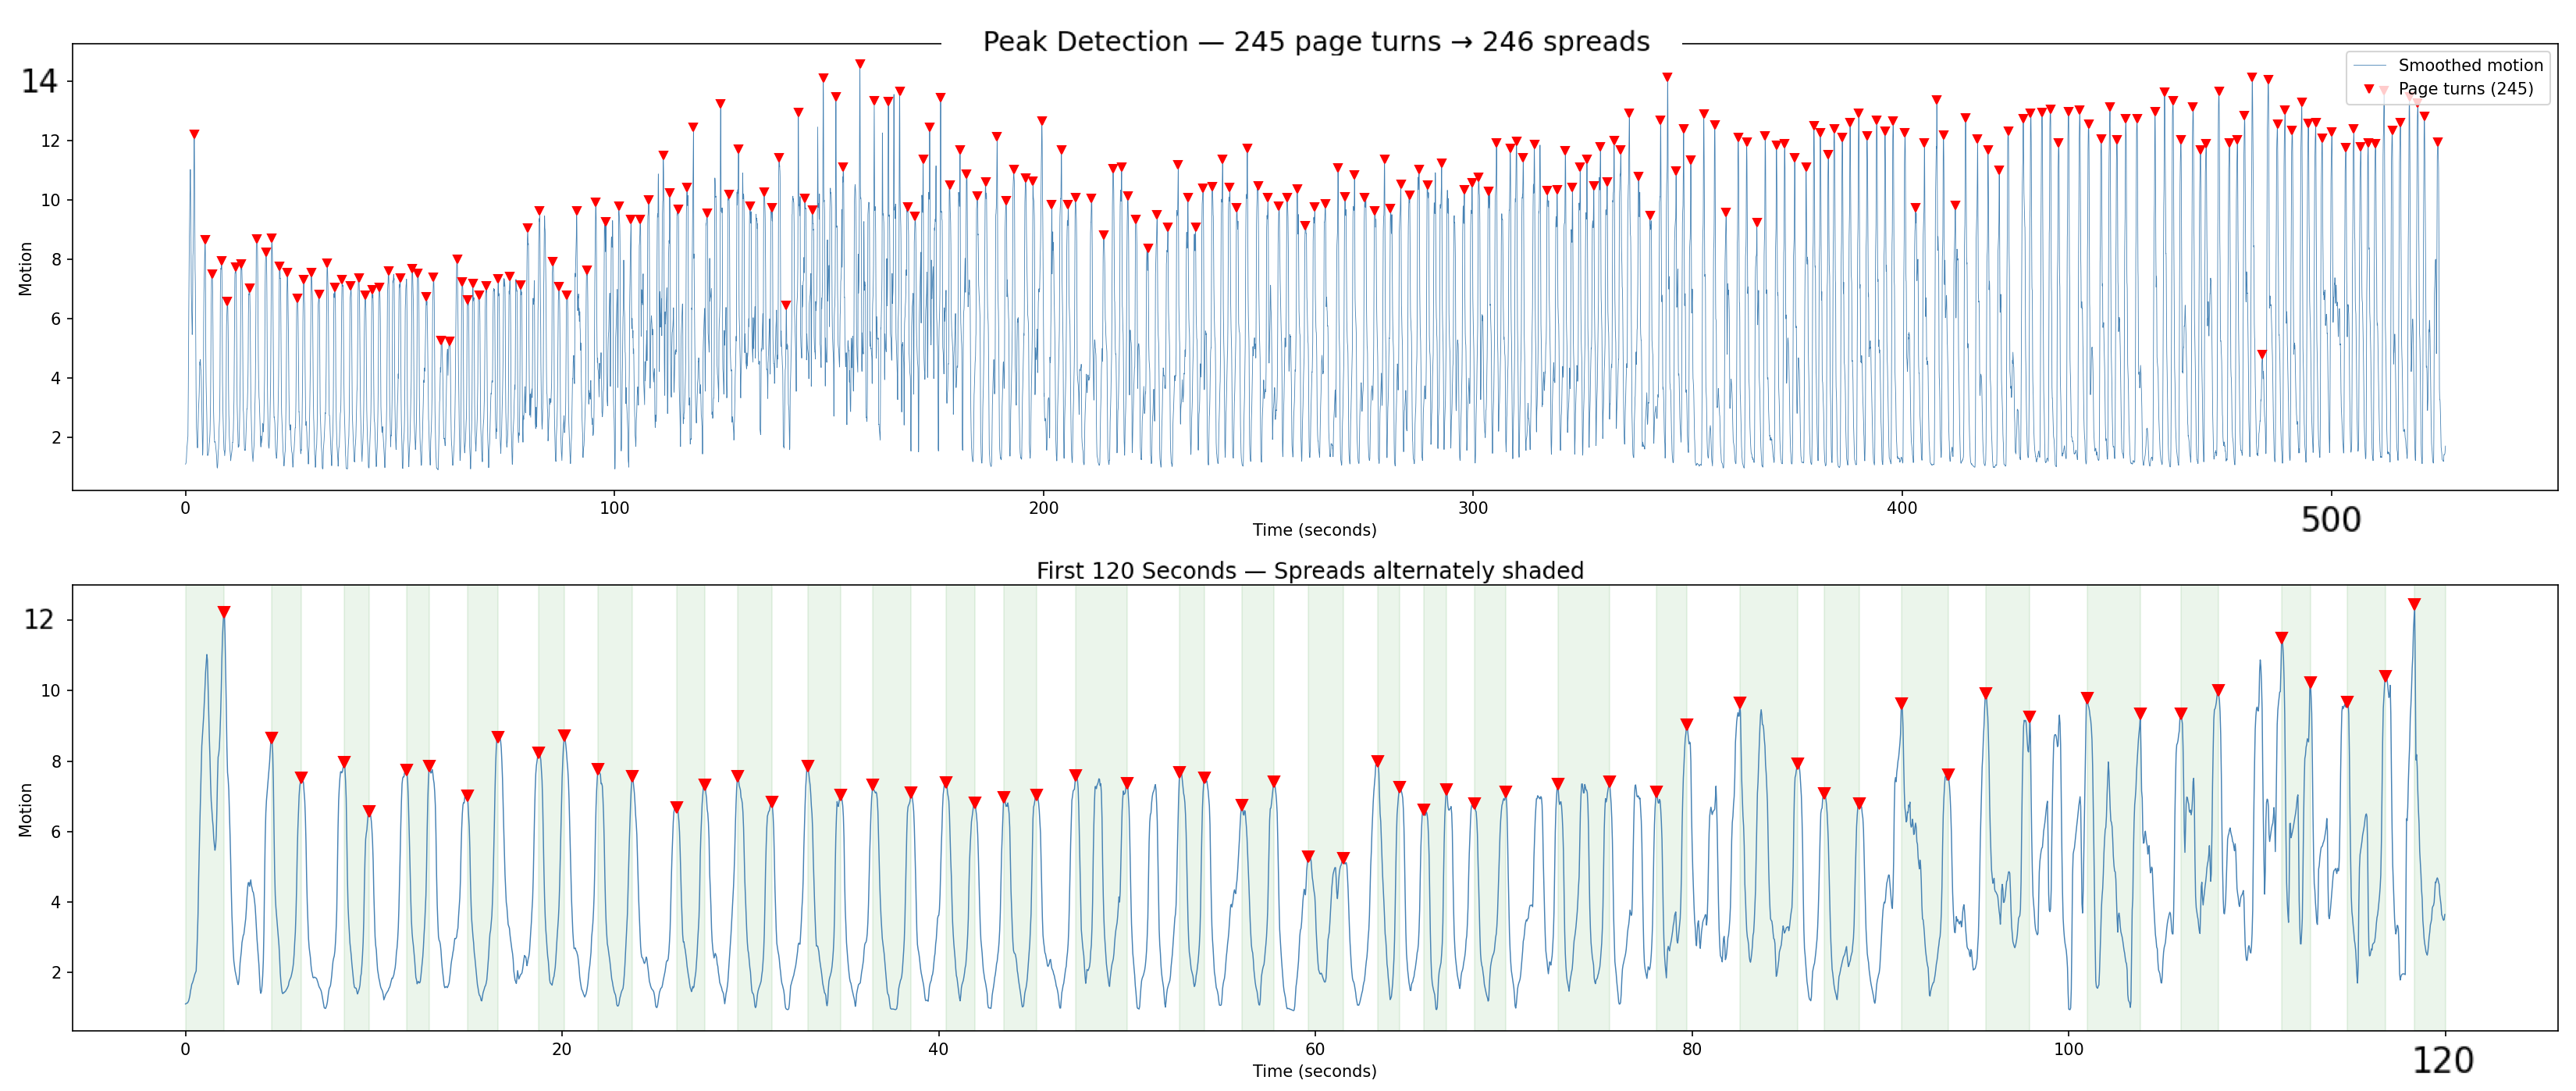
\includegraphics[width=0.97\linewidth]{images/peaks_plot2.png}
%     \caption{Motion-based page-turn detection on a representative book scan. The
%     top panel shows the smoothed motion signal over the full recording, with
%     detected peaks marked as page turns; the detector identifies $245$ page
%     turns, corresponding to $246$ scanned spreads. The bottom panel zooms into
%     the first $120$ seconds, where alternating shaded bands indicate successive
%     spreads and red markers show detected page-turn events (mean spread
%     duration $\approx 2$\,seconds).}
%     \label{fig:peaks}
% \end{figure*}

\subsection{Offline Keyframe Extraction}
\label{sec:offline}

\sys also accepts a \emph{pre-recorded} video---archival footage, or a book
filmed on a phone away from the workstation---and recovers the same per-spread
keyframes in a batch pass over the finished recording. With the whole signal in
hand at once, the offline path can segment more deliberately than the causal live
machine, detecting page turns globally rather than committing to each one as it
happens.

\noindent\textbf{Phase 1 --- Motion signal.}
\sys computes the same inter-frame motion of Equation~\ref{eq:motion} over every
frame of the recording, now smoothed with a \emph{centered} 15-frame moving
average $\tilde{m}_t$ (offline, a symmetric window is available). A single
sequential read at reduced resolution processes a full-length recording cheaply,
while the averaging suppresses per-frame sensor noise without blurring the
page-turn bursts.

\noindent\textbf{Phase 2 --- Page-turn detection.}
Page turns appear as peaks in $\tilde{m}_t$. We extract them with
\texttt{scipy.signal.find\_peaks}~\cite{virtanen2020scipy}, requiring a minimum
height, a minimum inter-peak spacing of $1.5$\,s, and a minimum prominence so
that text-density flicker within a settled spread is not mistaken for a turn.
Consecutive peaks bound the per-spread intervals. A second pass rescues fast
double-turns that the first pass merges: any interval longer than $3$\,s is
rescanned for two stillness valleys (motion below threshold for at least
$0.15$\,s) bracketing a motion bump, the signature of a second turn that was
flipped through quickly, and the bump is inserted as an additional boundary.
Figure~\ref{fig:peaks} shows the result on a representative book: $245$ detected
page turns yield $246$ spreads, with a mean spread duration of roughly
$2$\,seconds.

\noindent\textbf{Phase 3 --- Keyframe selection.}
Within each spread interval, \sys selects a single representative frame. The
candidates are the \emph{stillest} frames---those whose smoothed motion falls
within a small margin of the interval minimum. Among these, the frame with the
highest sharpness wins, measured as the variance of the Laplacian over the
central $80\%$ of the frame (the margins are excluded so that a hand or page edge
entering the border does not inflate the score). The chosen frame is then
extracted from the source video at full resolution and written to disk. Stillness
picks the moment the spread lies flat and motion-free; sharpness then breaks ties
among those still frames, discarding any in which the autofocus has not finished
settling.

\subsection{Review, Crop, and Assembly}
\label{sec:backhalf}

Both front ends converge on a shared back half that turns the per-spread
keyframes into a finished PDF. One stage is interactive (P4) and the rest are
automated, with an optional second review (P7) and binarization pass (P8).

\noindent\textbf{Phase 4 --- Keyframe review.}
An interactive interface presents the selected keyframes in order. The operator
deletes low-quality or duplicate frames, inserts any spread the detector missed
(via a frame scrubber over the source video), tags front and back covers, and
adjusts per-spread geometry. The geometry editor adapts to the capture mode: for
book spreads it exposes the split (gutter) line and a deskew angle; for loose
single documents it exposes an adjustable, rotatable crop box. Crucially, a
manual correction propagates \emph{forward} as a prior to later spreads---the
rig does not move between page turns, so one adjustment typically fixes a long
run of frames---which keeps correction the exception rather than a per-frame
chore. The phase is reentrant and can be revisited as many times as needed
before proceeding.

\noindent\textbf{Phase 5 --- Crop.}
Cropping isolates the book from the surrounding table. A grayscale Otsu
threshold~\cite{otsu1979threshold} fails here because cream-colored pages and a
light-brown wooden table overlap in luminance and merge into one region.
Instead, \sys builds the page mask in HSV space, keeping regions of low
saturation and high value: a page is bright and nearly colorless, whereas a
tinted table is darker and more saturated, and the distinction is invariant to
where the spread sits or how it is rotated. From this mask the spread's tilt is
estimated by a robust (Huber) line fit to its top edge and corrected by
rotation; the page is then tight-cropped to the mask bounds, with thin
protrusions---a finger, or an underlying page poking past the edge---rejected by
keeping only the rows and columns whose page coverage exceeds half the peak. For
loose single documents, \sys instead segments the page from the table with
GrabCut~\cite{rother2004grabcut} and perspective-warps the resulting
quadrilateral to a straight rectangle; an operator's manual crop box from review
overrides the automatic detection when page sizes vary.

\noindent\textbf{Phase 6 --- Split.}
Book spreads are split into two pages at the gutter. Rather than scanning for the
faint shadow valley between the pages---which a per-column brightness scan
readily confuses with a text-block edge---\sys places the spine at the book's
geometric center, the row-wise median of the midpoint between the detected left
and right page edges. Because a bound book's two pages are equal width, this
midpoint is exactly where the spine lies, and it tracks the book steadily as it
shifts in the frame. Manual gutter corrections from review act as priors: near a
prior, the spine is re-tracked in a tight band but only follows a column that is
a genuine shadow (measurably darker than the surrounding band). Each resulting
half then receives a fine text-line deskew via a projection-profile search, since
page curvature near the spine can skew the two halves differently.

\noindent\textbf{Phase 7 --- Page quality review (optional).}
A second interactive pass lets the operator inspect the final pages, flag issues
such as crop errors or poor focus, and drop bad ones; the annotations save to a
shareable report that can guide later algorithmic improvement.

\noindent\textbf{Phase 8 --- Binarization (optional).}
For text-heavy documents on thick paper, \sys can produce clean black-and-white
pages. Naive thresholding looks grainy, but the grain is a pipeline
artifact---coarse-grid edge quantization at native width, plus JPEG ringing---not
the threshold itself. \sys therefore upscales the grayscale (cubic) to anti-alias
contours, applies Sauvola local thresholding~\cite{sauvola2000adaptive} (robust to
the gutter-shadow gradient a Gaussian threshold smears into blotches), de-speckles
with a stroke-preserving $3\times3$ median, and writes lossless PNG. Not
recommended for pages with photographs or colored backgrounds.

\noindent\textbf{Phase 9 --- PDF assembly.}
Finally, the page images are assembled in order into a PDF, each page sized to
match the aspect ratio of its source image. Binarized pages are embedded
losslessly (as bitonal CCITT/Flate) rather than re-encoded as JPEG, which would
reintroduce the very ringing that careful binarization removes.

% When merging into the full paper, drop these two lines and let the main
% document's bibliography resolve these keys (switch to the ACM style).
\bibliographystyle{plain}
\bibliography{references}

\end{document}
